\documentclass{ieeeaccess}
\usepackage{cite}
\usepackage{amsmath,amssymb,amsfonts}
\usepackage{algorithmic}
\usepackage{graphicx}
\usepackage{textcomp}
\usepackage{booktabs}
\usepackage{placeins}
\usepackage{url}

\usepackage{bm}
\makeatletter
\AtBeginDocument{\DeclareMathVersion{bold}
\SetSymbolFont{operators}{bold}{T1}{times}{b}{n}
\SetSymbolFont{NewLetters}{bold}{T1}{times}{b}{it}
\SetMathAlphabet{\mathrm}{bold}{T1}{times}{b}{n}
\SetMathAlphabet{\mathit}{bold}{T1}{times}{b}{it}
\SetMathAlphabet{\mathbf}{bold}{T1}{times}{b}{n}
\SetMathAlphabet{\mathtt}{bold}{OT1}{pcr}{b}{n}
\SetSymbolFont{symbols}{bold}{OMS}{cmsy}{b}{n}
\renewcommand\boldmath{\@nomath\boldmath\mathversion{bold}}}
\makeatother

\def\BibTeX{{\rm B\kern-.05em{\sc i\kern-.025em b}\kern-.08em
    T\kern-.1667em\lower.7ex\hbox{E}\kern-.125emX}}

% Allow more floats per page and reduce float deferral
\renewcommand{\topfraction}{0.9}
\renewcommand{\bottomfraction}{0.9}
\renewcommand{\textfraction}{0.1}
\renewcommand{\floatpagefraction}{0.8}
\setcounter{topnumber}{4}
\setcounter{bottomnumber}{4}
\setcounter{totalnumber}{8}

\begin{document}
\vol{13}
\year{2025}
\history{Date of publication xxxx 00, 0000, date of current version xxxx 00, 0000.}
\doi{} % DOI to be assigned by IEEE Access production

\title{SE-Blackboard: A Shared-State Architecture for Multi-Agent Software Engineering Pipelines}
\author{\uppercase{Erxi Liu}\authorrefmark{1},
\uppercase{Qiang Zhu}\authorrefmark{2},
\uppercase{Xinru Dong}\authorrefmark{3,2}}

\address[1]{Tandon School of Engineering, New York University, New York, United States (e-mail: el4435@nyu.edu)}
\address[2]{The National Institute of Metrology of China, Beijing, China (e-mail: zhuqiang@nim.ac.cn)}
\address[3]{School of Mechanical and Electrical Engineering, Beijing Institute of Graphic Communication, Beijing, China (e-mail: 18339301370@163.com)}

\markboth
{Liu \headeretal: SE-Blackboard: A Shared-State Architecture for Multi-Agent SE Pipelines}
{Liu \headeretal: SE-Blackboard: A Shared-State Architecture for Multi-Agent SE Pipelines}

\corresp{Corresponding author: Qiang Zhu (e-mail: zhuqiang@nim.ac.cn).}

\begin{abstract}
Multi-agent large language model (LLM) systems are increasingly used for software engineering tasks, yet the role of \textbf{communication architecture} in these systems remains poorly understood. Most existing approaches rely on message passing, where agents communicate through sequential natural language summaries, potentially introducing information loss across pipeline stages. This paper introduces \textbf{SE-Blackboard}, a modular framework that applies a shared-state Blackboard architecture to multi-agent software engineering pipelines. We conduct controlled experiments on 50 SWE-bench Lite issues, comparing three communication architectures: message passing, shared-state blackboard, and a hybrid design. Our results show that communication architecture significantly affects information preservation and intermediate pipeline performance. The blackboard configuration improves Coder-stage information fidelity (IFS) by 62\% compared with message passing (0.586 vs. 0.362), which translates into a 27.5 percentage-point improvement in correct file targeting (82.6\% vs. 55.1\%). However, once the correct file is identified, all configurations converge to a $\sim$22\% conditional resolve rate, revealing a downstream bottleneck in LLM diff generation. As a result, the overall resolve-rate improvement is modest (16\% vs. 12\%) despite large upstream gains. These findings highlight communication architecture as an important design dimension for multi-agent software engineering systems and suggest that improvements in upstream information quality translate into task-level gains only when downstream generation bottlenecks are addressed.
\end{abstract}

\begin{keywords}
multi-agent systems, large language models, software engineering, blackboard architecture, shared state, communication architecture, information fidelity, SWE-bench
\end{keywords}

\titlepgskip=-21pt

\maketitle

\section{Introduction}

\PARstart{T}{he} rapid advancement of large language models (LLMs) \cite{brown2020language} has catalyzed the emergence of multi-agent systems for software engineering (SE). Systems such as MetaGPT \cite{hong2024metagpt}, ChatDev \cite{qian2024chatdev}, SWE-Agent \cite{yang2024sweagent}, and AgentCoder \cite{huang2024agentcoder} demonstrate that multiple AI agents can collaboratively solve complex tasks, including code generation \cite{chen2021evaluating}, bug fixing, and code review, representing a shift from monolithic tools toward modular, role-based architectures.

However, current multi-agent SE systems share a common architectural assumption: \textbf{message-passing communication}. Agents communicate by forwarding natural-language messages along a predefined chain; the output of one agent becomes the input to the next. This approach has a fundamental limitation: information fidelity degrades at each handoff. Critical technical information, such as function signatures, parameter types, and error stack traces, may be paraphrased, simplified, or omitted. We term this progressive degradation of information \emph{knowledge drift}, which has also been identified as a primary failure cause in multi-agent LLM systems \cite{cemri2025why}.

Knowledge drift is particularly critical in software engineering contexts. While paraphrasing in general reasoning tasks may preserve semantic equivalence, SE tasks require exact technical precision. A single character difference in a function name or file path can determine whether a patch applies correctly, making SE an ideal domain for studying information preservation in multi-agent architectures.

Existing approaches to communication quality have focused on post-hoc remediation. RTADev \cite{fang2025rtadev} proposes intention alignment to verify that agents' interpretations match the original intent, but only detects information loss after it has occurred. The Blackboard architecture, on the other hand, offers an alternative. It is a classical AI pattern featuring a shared workspace accessible to all agents \cite{nii1986blackboard}. Recent work has demonstrated Blackboard's effectiveness for LLM-based reasoning \cite{wang2025lbmas} and data science \cite{salemi2025llm} tasks, but it has never been applied to software engineering.

This paper makes the following contributions:

\begin{enumerate}
\item \textbf{SE-Blackboard Framework}: The application of the Blackboard shared-state architecture to multi-agent software engineering, which includes three pluggable communication modes (Message-Passing, Blackboard, and Hybrid) within identical agent pipelines.

\item \textbf{Information Fidelity Score (IFS)}: A new metric that measures the preservation of key technical entities across pipeline stages, enabling measurement of information preservation independent of downstream task success.

\item \textbf{Controlled Empirical Evaluation}: Experiments on 50 SWE-bench Lite issues demonstrate that BB improves Coder-stage IFS by 62\% (0.586 vs. 0.362, $p=0.058$) and resolve rate by 4 percentage points (16\% vs. 12\%), with patch formatting identified as the primary bottleneck.

\item \textbf{Open-Source Framework}: A modular framework with pluggable communication architectures, structured state schemas, and comprehensive logging for future research.

\end{enumerate}
\section{Related Work}

\subsection{Multi-Agent Systems for Software Engineering}

Recent studies have introduced a range of multi-agent software engineering (SE) systems that differ in architectural design and interaction style, which typically rely on the code-generation strengths of foundation models such as Codex \cite{chen2021evaluating} and Code Llama \cite{roziere2023code}. Role-oriented frameworks---such as MetaGPT \cite{hong2024metagpt}, ChatDev \cite{qian2024chatdev}, and AutoGen \cite{wu2023autogen}---assign specialized responsibilities to individual agents and organize their collaboration through predefined workflows or structured dialogue. In contrast, tool-augmented approaches such as SWE-Agent \cite{yang2024sweagent} and AutoCodeRover \cite{zhang2024autocoderover} focus on enhancing a single agent with repository navigation and execution tools, achieving strong performance without explicit multi-agent coordination.

For automated bug fixing, AgentCoder \cite{huang2024agentcoder} and CodeR \cite{chen2024coder} use multi-agent pipelines that incorporate iterative feedback from test execution, whereas Agentless \cite{xia2024agentless} shows that carefully designed prompting strategies can attain comparable results without deploying multiple agents. This comparison suggests that interaction design may be as influential as agent multiplicity itself.

Despite their differences, these systems largely rely on message passing as the primary mechanism for inter-agent communication. Although some approaches use shared artifacts, the communication architecture is seldom examined as an independent design dimension. Our work seeks to fill this gap.

\subsection{Communication Architectures for LLM Agents}

He et al.~\cite{he2025llm} provide a survey of LLM-based multi-agent systems for software engineering, outlining several communication patterns, including direct messaging, shared memory, and blackboard-style coordination. They observe, however, that many existing systems still rely on relatively simple sequential exchanges. Cemri et al.~\cite{cemri2025why} examine common failure modes in multi-agent LLM systems and identify knowledge drift as a central issue, showing that drift becomes more evident as the length of agent interaction chains increases.

Alongside research on communication architectures, recent studies focus on strengthening the reasoning abilities of individual agents in multi-agent settings. Chain-of-Thought prompting \cite{wei2022chain} supports stepwise reasoning, while ReAct \cite{yao2023react} integrates reasoning with tool use, grounding agent decisions in environmental feedback. Reflexion \cite{shinn2023reflexion} introduces a verbal reinforcement-learning framework that enables agents to iteratively refine their behavior by reflecting on prior mistakes. Park et al.~\cite{park2023generative} further demonstrate that generative agents with memory and reflective mechanisms can display coherent collaborative behavior, providing a firm basis for more advanced coordination strategies.

More recently, RTADev \cite{fang2025rtadev} introduces intention alignment as a reactive mechanism that mitigates information loss after it occurs. By contrast, the Blackboard architecture adopted in our work takes a proactive approach, ensuring that all agents retain direct access to source information regardless of intermediate processing steps.

\subsection{Blackboard Architecture}

The Blackboard architecture, first introduced by Nii~\cite{nii1986blackboard}, describes a framework in which multiple knowledge sources coordinate through a shared workspace, which was initially applied to speech understanding and planning systems \cite{erman1980hearsay}. Recently, this framework has attracted further interest in the context of LLM-based multi-agent coordination. Wang et al.~\cite{wang2025lbmas} show that communication through a shared state can reduce information loss compared with message passing in reasoning tasks, and the benefits become more evident as task complexity and the length of agent interaction chains increase. Salemi et al.~\cite{salemi2025llm} explore this pattern in data science workflows and report improved coherence when agents can directly observe each other's outputs.

To our knowledge, this work brings the approach to software engineering for the first time. Software engineering tasks introduce additional challenges: the system state must capture heterogeneous artifacts such as issue descriptions, code context, patches, and test results while maintaining clear ownership semantics. Moreover, code-related information requires a much higher degree of precision than typical natural language reasoning.

\section{System Design}

SE-Blackboard is a modular framework that aims to study how communication architecture affects performance on software engineering tasks. As shown in Figure~\ref{fig:architecture}, the system consists of four main components: a structured state schema, three interchangeable communication modes, four specialized agents, and a pipeline-based topology.

\begin{figure*}[t]
\centering
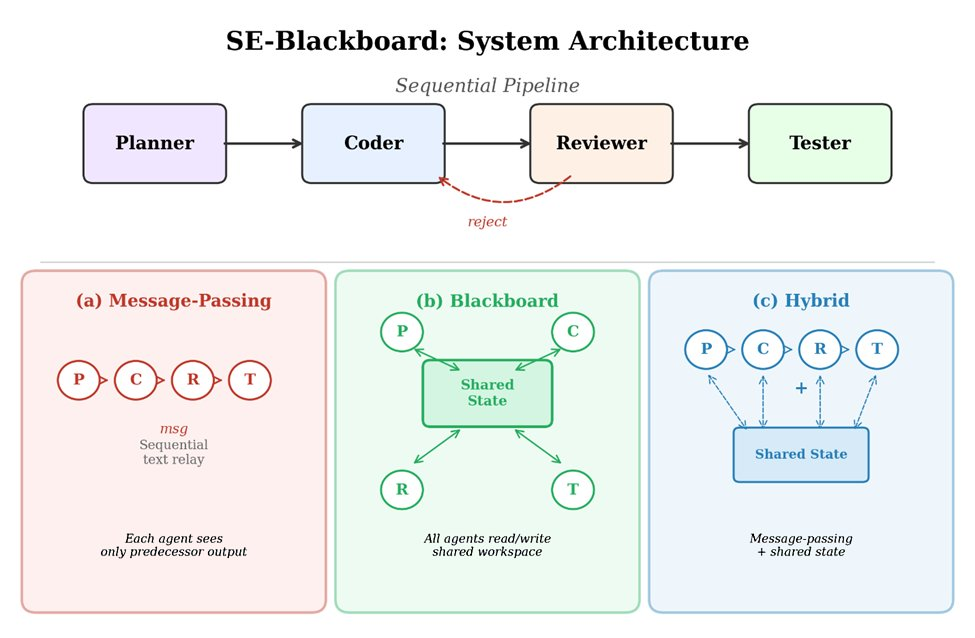
\includegraphics[width=\textwidth]{figures/fig1_SE-Blackboard_modified.png}
\caption{SE-Blackboard system architecture. The framework consists of a structured state schema, three interchangeable communication modes (Message-Passing, Blackboard, Hybrid), four specialized agents, and a sequential pipeline topology.}
\label{fig:architecture}
\end{figure*}

\subsection{SE State Schema}

The framework uses a domain-specific state schema implemented as Pydantic models to represent the key artifacts produced during the bug-fixing pipeline, including \textbf{IssueInfo} (the original issue description, repository, and base commit), \textbf{Analysis} (the Planner's root-cause analysis and proposed fix strategy), \textbf{Patch} (the Coder's generated unified diff), \textbf{Review} (the Reviewer's accept/reject decision along with feedback), and \textbf{TestResult} (the Tester's pass/fail evaluation).

Formally, the shared state is defined as a tuple:

\[\mathbf{S} = (I, A, P, R, T)\]

where \emph{I} denotes IssueInfo, \emph{A} denotes Analysis, \emph{P} denotes Patch, \emph{R} denotes Review, and \emph{T} denotes TestResult.

A key design principle is \textbf{field ownership}. Each agent is only allowed to write to its designated state fields and has read access to upstream fields. The write-permission mapping $W$ is defined as follows:

\begin{align*}
W(\text{Planner}) &= \{A\}, \quad W(\text{Coder}) = \{P\}, \\
W(\text{Reviewer}) &= \{R\}, \quad W(\text{Tester}) = \{T\}
\end{align*}

This ownership model prevents agents from inadvertently overwriting each other's contributions and ensures a clear audit trail.

Crucially, the original issue description (IssueInfo) is always preserved in the shared state and remains directly accessible to all agents. This design mitigates knowledge drift: downstream agents, such as the Coder, can reference the original issue text directly rather than relying solely on the Planner's summarization.

\subsection{Communication Modes}
\label{sec:comm-modes}

The framework supports three communication modes (Figure~\ref{fig:architecture}, bottom):

\textbf{Message-Passing (MP)}: Each agent receives only the output of its immediate predecessor as natural language input and does not share structured state. This configuration reflects many existing multi-agent SE systems.

\textbf{Blackboard (BB)}: All agents read from and write to a shared state instance. Each agent is provided with a role-specific view through \texttt{get\_state\_for\_agent(role)}, which includes all upstream fields together with the original issue description. The Coder receives both the Planner's structured analysis \emph{and} the original issue text, enabling cross-referencing.

\textbf{Hybrid}: Agents have access to both message-passing context and the shared blackboard state, combining the two information channels.

We formalize the modes using a context function $C(k)$, which specifies the information available to the $k$-th agent at execution time. Let $\text{out}(k{-}1)$ denote the natural language output of the preceding agent, $S_j$ denote the state field written by agent $j$, and $I$ denote the original issue description.

\textbf{Message-Passing:}

\[C^{\text{MP}}(k) = \{\text{out}(k{-}1)\}\]

\textbf{Blackboard:}

\[C^{\text{BB}}(k) = \{S_j \mid j < k\} \cup \{I\}\]

\textbf{Hybrid:}

\[C^{\text{Hy}}(k) = \{\text{out}(k{-}1)\} \cup \{S_j \mid j < k\} \cup \{I\}\]

The key architectural difference is that $I \in C^{\text{BB}}(k)$ and $I \in C^{\text{Hy}}(k)$ but $I \notin C^{\text{MP}}(k)$ for downstream agents ($k \geq 2$). In BB mode, the Coder always has direct access to the original issue text. On the other hand, in MP mode, the Coder obtains information about the issue only through the Planner's summarized output $\text{out}(\text{Planner})$. This distinction is the formal basis for the differences in information fidelity analyzed in Section~\ref{sec:ifs-results}.

All three modes share identical agent implementations and prompt templates, with only the context formatting varying by communication mode, ensuring that observed differences are attributable to the communication architecture.

\subsection{Agent Design}

The pipeline consists of four agents: \textbf{Planner}, \textbf{Coder}, \textbf{Reviewer}, and \textbf{Tester}. The Planner analyzes the issue to produce a root cause analysis and a fix strategy. The Coder generates a unified diff patch from the analysis and repository source code. The Reviewer evaluates the patch and provides accept/reject feedback, using a feedback-driven iteration mechanism similar to Reflexion \cite{shinn2023reflexion}. Finally, the Tester evaluates the resulting patch using the SWE-bench Docker harness. Each agent uses prompt variants tailored to the communication mode.

\begin{figure*}[t]
\centering
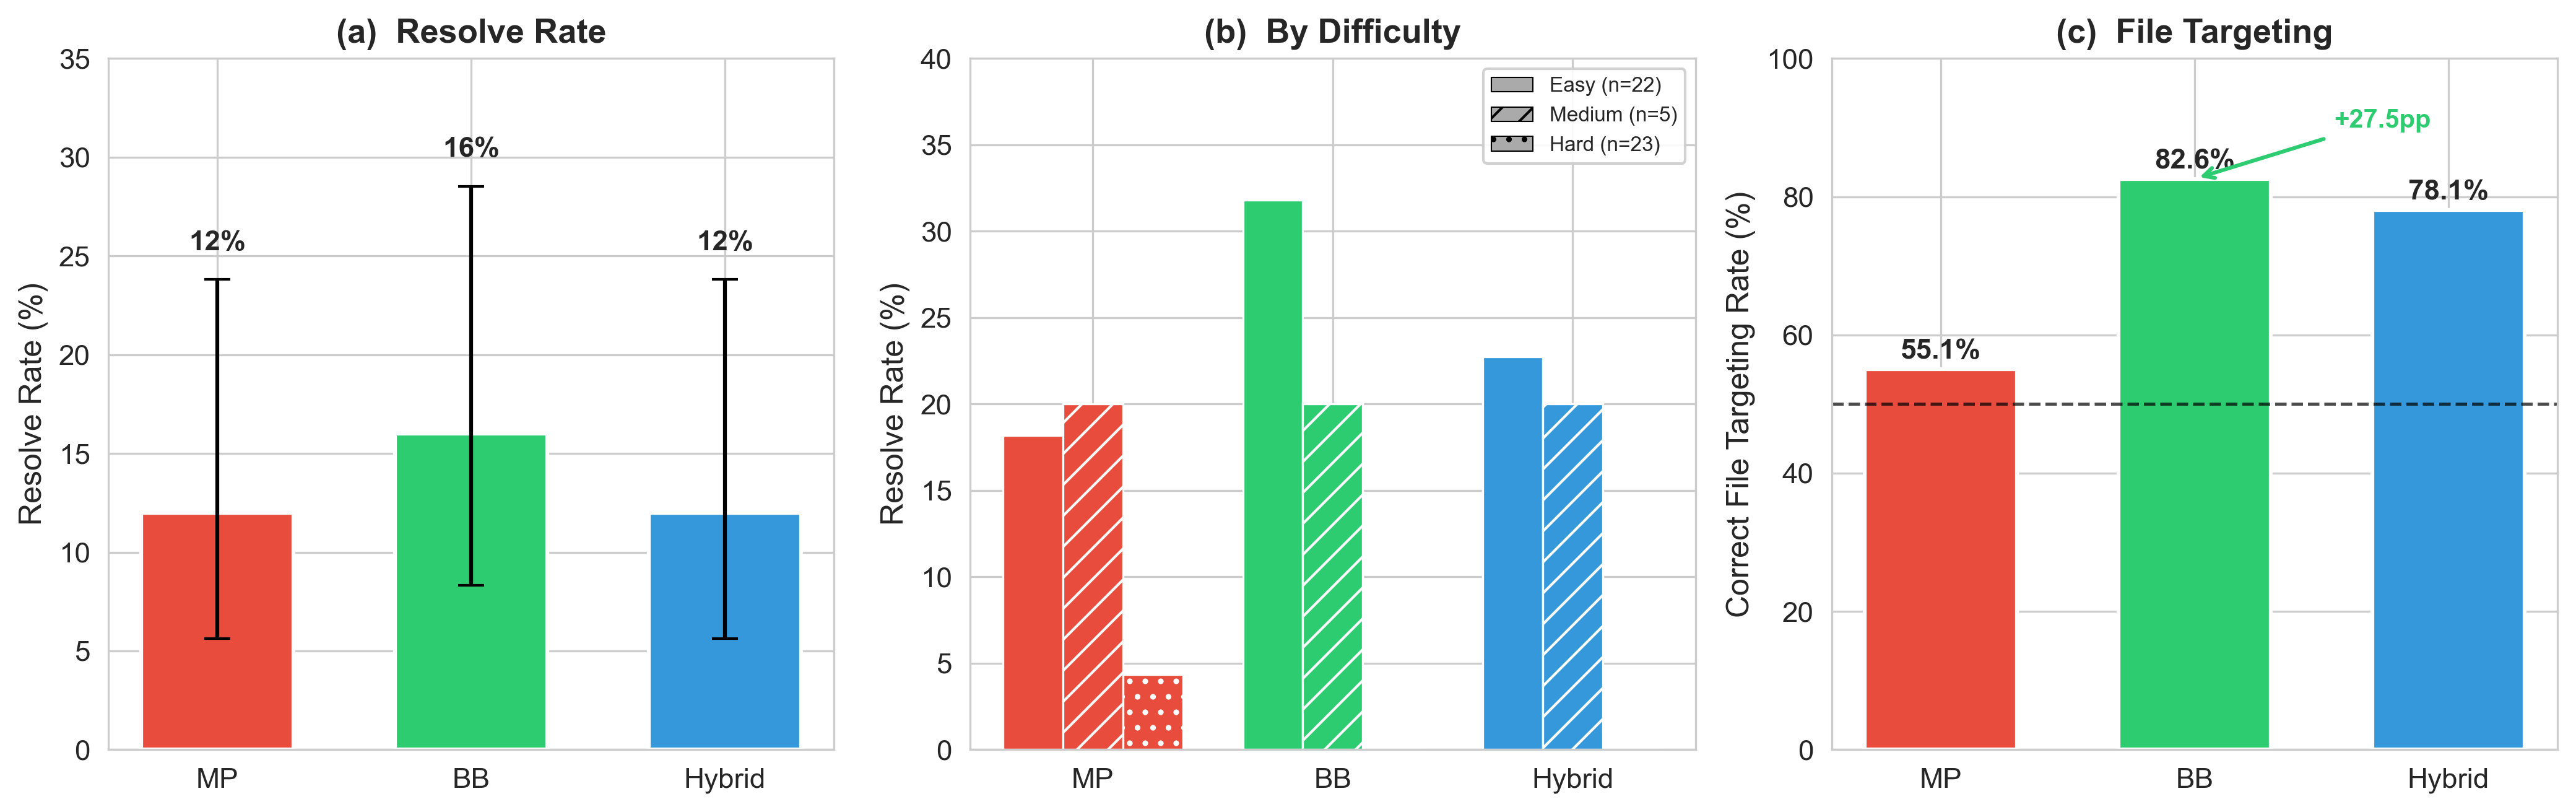
\includegraphics[width=\textwidth]{figures/fig2_main_results_panel.png}
\caption{Main experimental results. (a) Overall resolve rate by communication mode. (b) Resolve rate by difficulty level. (c) Correct file targeting rate among non-empty patches.}
\label{fig:main-results}
\end{figure*}

\subsection{Pipeline Topology}

The framework follows a sequential pipeline with a rejection loop from the Reviewer back to the Coder (up to 3 iterations). Once the patch is accepted or the maximum number of iterations is reached, the Tester evaluates the resulting patch. The Tester always executes regardless of the Reviewer's decision, ensuring that each run produces a test result.

Formally, let $\mathcal{P}$, $\mathcal{C}$, $\mathcal{R}$, and $\mathcal{T}$ denote the Planner, Coder, Reviewer, and Tester agents, respectively, and let $N$ denote the maximum number of Coder--Reviewer iterations. The pipeline output is:

\[\text{output} = \mathcal{T} \circ \left(\mathop{\circledcirc}\limits_{n=1}^{N} \mathcal{R} \circ \mathcal{C}\right) \circ \mathcal{P}(I)\]

where the inner loop terminates early if $\mathcal{R}$ returns an accept decision at iteration $n < N$.

\section{Experimental Setup}

\subsection{Benchmark}

We evaluate on SWE-bench Lite \cite{jimenez2024swebench}, which is a curated subset of 300 real-world GitHub issues from 12 popular Python repositories. Each issue includes a natural language problem description, a base commit, and test cases that the fix must pass (FAIL\_TO\_PASS) while not breaking existing functionality (PASS\_TO\_PASS).

We select a stratified sample of 50 issues to balance feasibility with coverage. Issues were initially sampled in equal strata based on repository metadata, then reclassified post-hoc using gold patch complexity as an objective difficulty proxy: Easy (single-file, $<$20 lines): 22 issues, predominantly Django; Medium (single-file, 20--50 lines or multi-file with small changes): 5 issues; Hard (multi-file, $>$50 lines, or complex reasoning): 23 issues. The final sample covers 8 repositories, with Django overrepresented (22/50) due to its comprehensive test coverage.

\subsection{Configurations}

We evaluate three configurations that combine the Sequential Pipeline with different communication modes:

\begin{table}[!ht]
\centering
\caption{Experimental configurations for the three communication modes.}
\label{tab:configurations}
\begin{tabular}{lll}
\toprule
\textbf{Configuration} & \textbf{Communication} & \textbf{Label} \\
\midrule
A-Seq(MP) & Message-Passing & MP \\
B-Seq(BB) & Blackboard & BB \\
C-Seq(Hy) & Hybrid & Hybrid \\
\bottomrule
\end{tabular}
\end{table}

All configurations use identical hyperparameters: Claude Sonnet 4.5 (claude-sonnet-4-5-20250929), temperature 0, a maximum of 3 Coder-Reviewer iterations, and function-level code context retrieved via git checkout. The single LLM with deterministic generation ensures that observed differences are attributable to the communication architecture. Each issue is evaluated once per configuration, yielding 150 total runs.

\subsection{Evaluation Metrics}

\textbf{Resolve Rate.} An issue is resolved if the generated patch causes all FAIL\_TO\_PASS tests to pass while maintaining PASS\_TO\_PASS tests. Evaluation is performed using the official SWE-bench Docker harness.

\textbf{Information Fidelity Score (IFS).} We extract key technical entities from the original issue (function names, class names, file paths, error types) using rule-based patterns, then measure the proportion of these entities that appear in each agent's output:

\[\text{IFS}_s = \frac{|\text{entities in agent } s\text{'s output}|}{|\text{entities in issue description}|}\]

In MP mode, IFS is computed only at the Coder stage; in BB and Hybrid modes, it is computed at all four stages. The rule-based extraction may undercount semantically equivalent references; Section~\ref{sec:threats} discusses this limitation.

\textbf{Patch Quality Metrics.} To localize the performance bottleneck, we analyze the patch generation rate (non-empty output), the correct-file targeting rate (the proportion of non-empty patches that modify the same file(s) as the gold patch), and the conditional resolve rate (among correct-file patches that pass evaluation).

\textbf{Efficiency Metrics.} We measure token consumption, latency, and iteration count per issue.

\subsection{Statistical Methods}

Given the paired design (each issue under all three configurations), we use McNemar's exact test \cite{mcnemar1947note} for resolve rate comparisons, Wilcoxon signed-rank test \cite{wilcoxon1945individual} for continuous measurements (tokens, latency, IFS), Cohen's $h$ for effect size, and odds ratio with 95\% CI. All tests use $\alpha = 0.05$. With $N=50$ and expected resolve rates of 12--16\%, statistical power to detect resolve-rate differences is limited; therefore, we interpret the results in conjunction with IFS and failure analysis.

\section{Results}

\begin{figure*}[t]
\centering
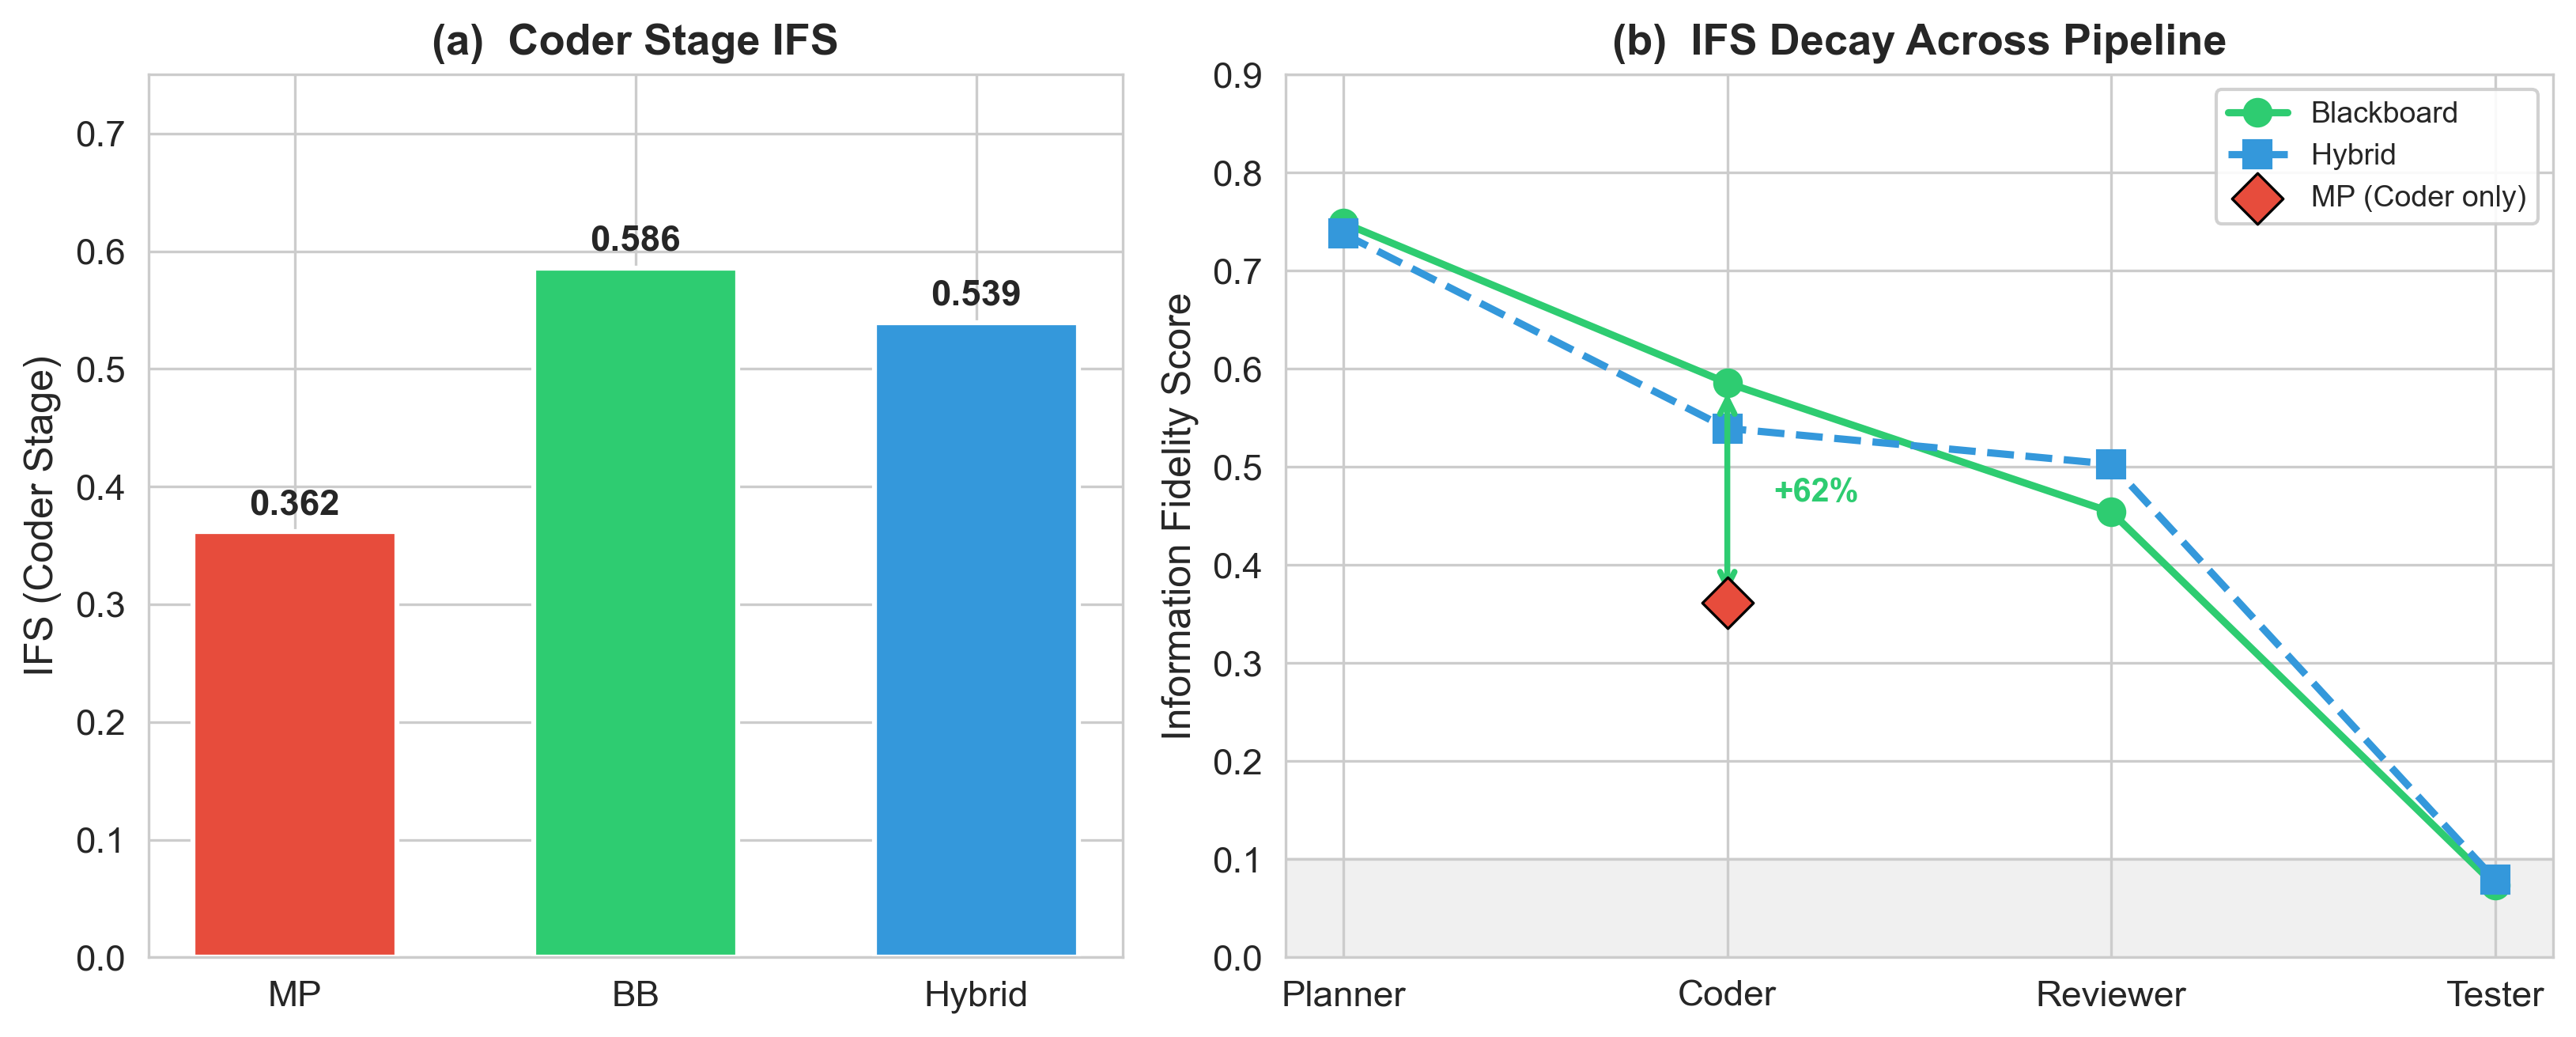
\includegraphics[width=\textwidth]{figures/fig3_ifs_analysis.png}
\caption{Information Fidelity Score (IFS) analysis. (a) Coder-stage IFS comparison between MP and BB. (b) IFS decay across pipeline stages for BB and Hybrid configurations.}
\label{fig:ifs-analysis}
\end{figure*}

\subsection{Resolve Rate}

Table~\ref{tab:main-results} presents the main experimental results across three communication architectures.

\begin{table}[!ht]
\centering
\caption{Main experimental results on SWE-bench Lite ($N=50$, Sequential pipeline).}
\label{tab:main-results}
\small
\begin{tabular}{lccccc}
\toprule
\textbf{Comm.} & \textbf{Res.} & \textbf{Rate} & \textbf{Tokens} & \textbf{Latency} & \textbf{Iter.} \\
\midrule
MP & 6/50 & 12.0\% & 25,316 & 106s & 2.78 \\
BB & 8/50 & 16.0\% & 54,849 & 171s & 2.70 \\
Hybrid & 6/50 & 12.0\% & 43,278 & 128s & 2.80 \\
\bottomrule
\end{tabular}
\end{table}

The Blackboard configuration resolves 8/50 issues (16.0\%), compared to 6/50 (12.0\%) for both MP and Hybrid, corresponding to a 4 percentage-point absolute improvement and 33\% relative improvement (Figure~\ref{fig:main-results}a). However, McNemar's exact test yields $p=0.625$ (see Table~\ref{tab:statistics} in Section~\ref{sec:stat-summary}) based on only 4 discordant pairs ($b=1$, $c=3$), indicating insufficient statistical power. Cohen's $h = 0.116$ confirms a negligible effect size, and the odds ratio of 1.40 (95\% CI [0.45, 4.37]) does not exclude the null hypothesis.

\subsubsection{Difficulty Breakdown}

The advantage of the Blackboard configuration is concentrated on easy-difficulty issues (Table~\ref{tab:difficulty}, Figure~\ref{fig:main-results}b). Among 22 easy issues, BB resolves 7 (31.8\%) compared with MP's 4 (18.2\%). In the medium category (5 issues), all configurations resolve exactly 1 (20.0\%). Among 23 hard issues, only MP resolves 1 (sphinx-8713, 4.3\%).

These results suggest that the information-preservation benefit of the Blackboard architecture is most apparent when the task falls within the agents' capability range.

\begin{table}[!ht]
\centering
\caption{Resolve rate by difficulty level.}
\label{tab:difficulty}
\begin{tabular}{lccc}
\toprule
\textbf{Difficulty} & \textbf{MP} & \textbf{BB} & \textbf{Hybrid} \\
\midrule
Easy (Django) & 4/22 (18.2\%) & 7/22 (31.8\%) & 5/22 (22.7\%) \\
Medium & 1/5 (20.0\%) & 1/5 (20.0\%) & 1/5 (20.0\%) \\
Hard & 1/23 (4.3\%) & 0/23 (0.0\%) & 0/23 (0.0\%) \\
\bottomrule
\end{tabular}
\end{table}

\subsubsection{Issue-Level Overlap}

Five issues form a "common core" resolved by all three configurations. BB uniquely resolves two additional issues (django-12915, django-13028); MP uniquely resolves sphinx-8713. In total, 9/50 issues (18\%) are resolved by at least one configuration.

\subsection{Information Fidelity Score}
\label{sec:ifs-results}

The IFS analysis provides clear evidence of the benefits of the Blackboard architecture (Table~\ref{tab:ifs}, Figure~\ref{fig:ifs-analysis}).

\begin{table}[!ht]
\centering
\caption{Average Information Fidelity Score by pipeline stage.}
\label{tab:ifs}
\begin{tabular}{lcccc}
\toprule
\textbf{Comm.} & \textbf{Planner} & \textbf{Coder} & \textbf{Reviewer} & \textbf{Tester} \\
\midrule
MP & N/A & 0.362 & N/A & N/A \\
BB & 0.749 & 0.586 & 0.454 & 0.074 \\
Hybrid & 0.738 & 0.539 & 0.503 & 0.079 \\
\bottomrule
\end{tabular}
\end{table}

\subsubsection{Coder Stage}

BB achieves an average Coder IFS of 0.586 compared to 0.362 under MP, resulting in a 62\% relative improvement (Wilcoxon W=36.5, p=0.058, n=28 non-zero pairs; Figure~\ref{fig:ifs-analysis}a). As mentioned in Section~\ref{sec:comm-modes}, the Coder's context under MP is $C^{\text{MP}}(\text{Coder}) = \{\text{out}(\text{Planner})\}$, whereas under BB it is $C^{\text{BB}}(\text{Coder}) = \{A, I\}$, which includes both the Planner's analysis and the original issue description $I$. Due to the absence of $I$ from $C^{\text{MP}}$, the Coder is forced to rely entirely on the Planner's lossy summarization, which accounts for the 62\% improvement in entity preservation.

\subsubsection{Information Decay Pattern}

For BB and Hybrid, IFS decays across the pipeline stages (Figure~\ref{fig:ifs-analysis}b): Planner ($\sim$0.74) $\rightarrow$ Coder ($\sim$0.56) $\rightarrow$ Reviewer ($\sim$0.48) $\rightarrow$ Tester ($\sim$0.08). This decline reflects a shift toward implementation tasks in downstream stages rather than reproducing terminology from the original issue description.

\subsubsection{IFS and Resolve Rate}

While a higher IFS does not guarantee resolution, the two issues uniquely resolved under BB (django-12915 and django-13028) both exhibit substantially higher Coder IFS compared with MP. This pattern suggests that improved information preservation may have contributed to their successful resolution.

\subsection{Failure Analysis}

Patch formatting, rather than information quality, appears to be the primary bottleneck across all configurations (Table~\ref{tab:failures}).

\begin{table}[!ht]
\centering
\caption{Failure mode distribution.}
\label{tab:failures}
\begin{tabular}{lccc}
\toprule
\textbf{Category} & \textbf{MP} & \textbf{BB} & \textbf{Hybrid} \\
\midrule
Resolved & 6 & 8 & 6 \\
Empty Patch & 1 & 4 & 18 \\
Patch Apply Error & 43 & 38 & 26 \\
\midrule
Total & 50 & 50 & 50 \\
\bottomrule
\end{tabular}
\end{table}

\textbf{Patch Apply Error} is the most common failure mode (MP: 43/50, BB: 38/50, Hybrid: 26/50), occurring when generated diffs contain context lines that do not match repository content.

\textbf{Empty Patch} failures are very frequent in Hybrid mode (18/50, 36\%) compared with MP (1/50, 2\%) and BB (4/50, 8\%), suggesting that the dual-channel context overwhelms the Coder.

The large gap between BB's IFS advantage (62\%) and its resolve rate advantage (4pp) is explained by this patch-formatting bottleneck; Section~\ref{sec:patch-quality-analysis} provides a fine-grained decomposition.

\begin{figure*}[t]
\centering
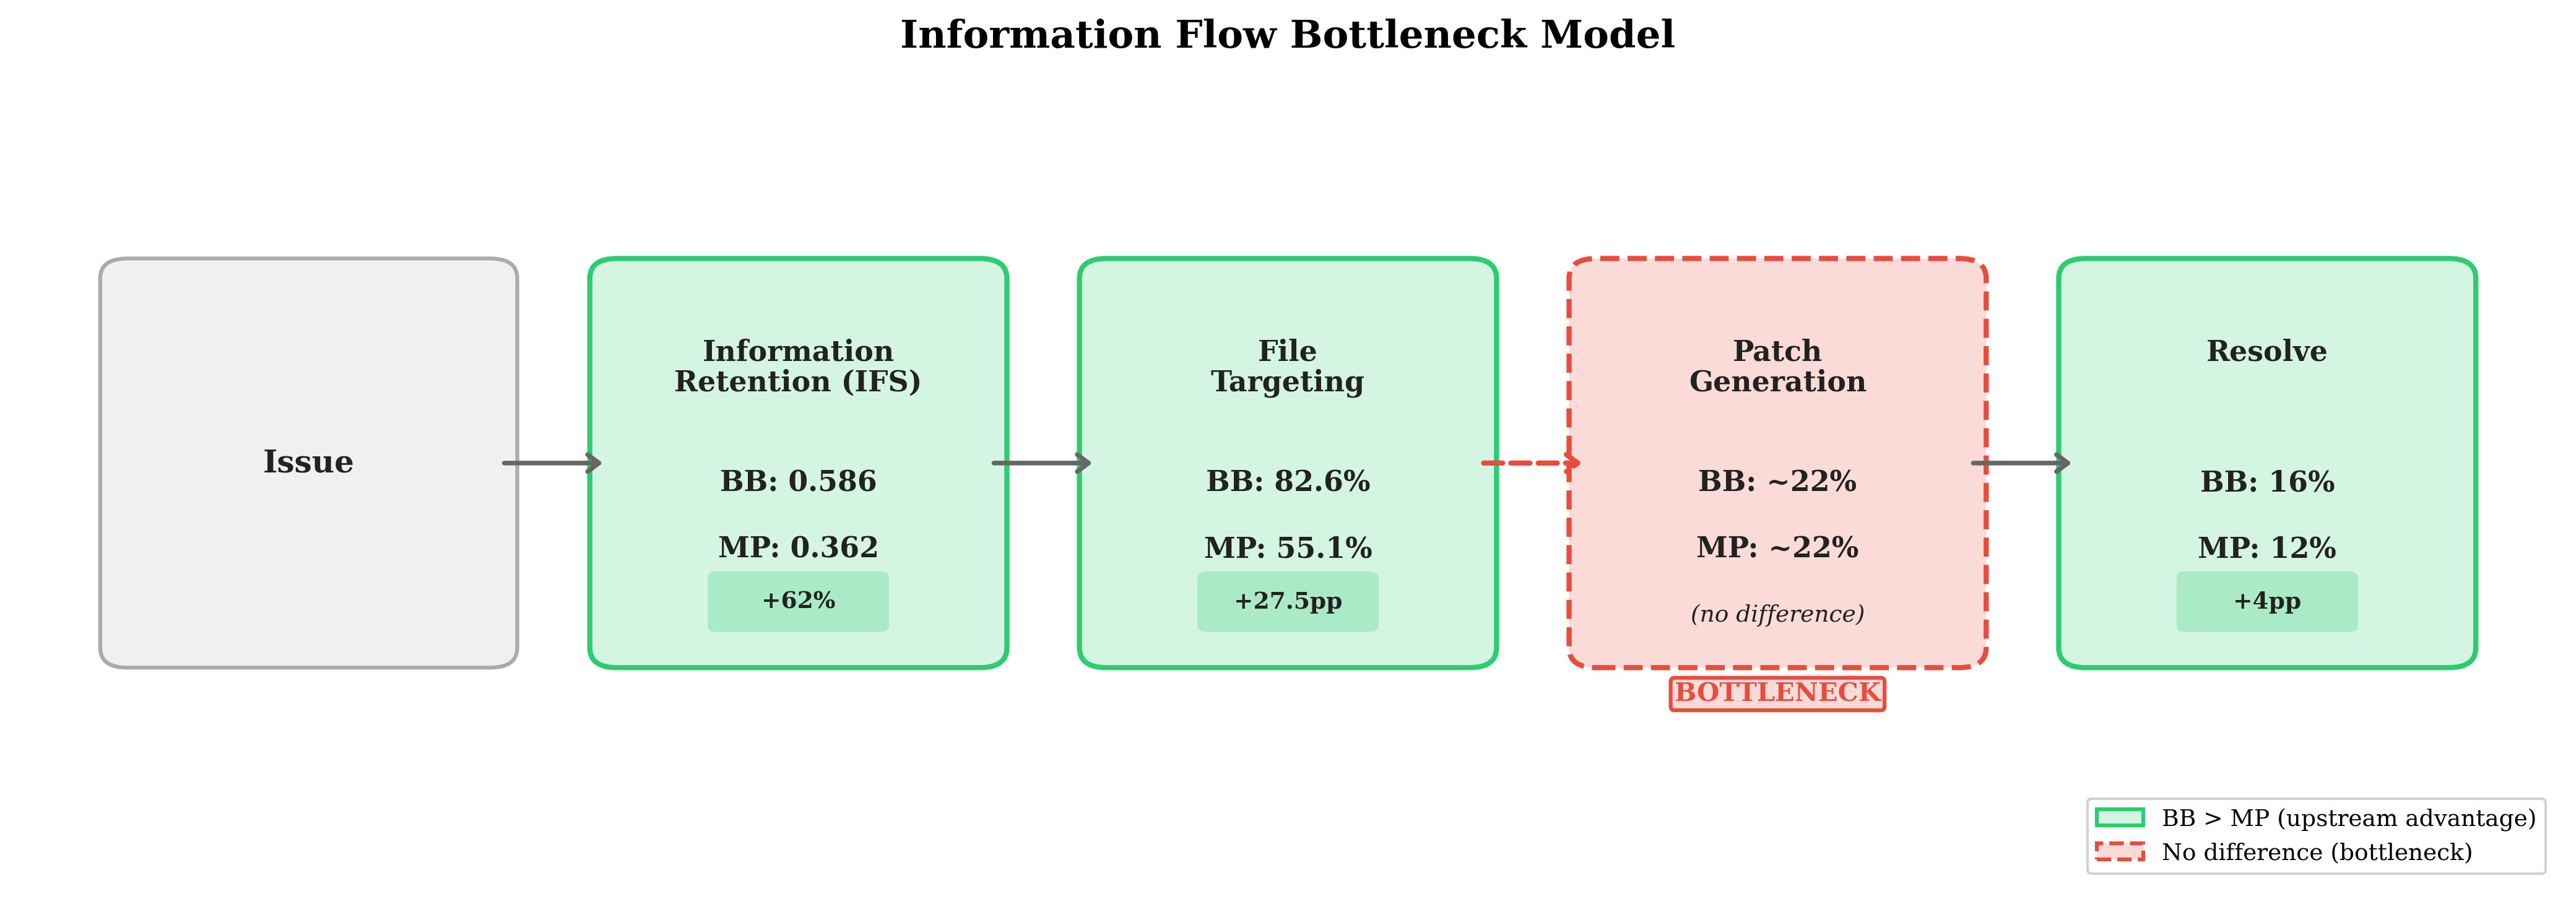
\includegraphics[width=\textwidth]{figures/fig4_bottleneck_model.png}
\caption{Information flow bottleneck model. BB outperforms MP in IFS and file targeting (upstream), but all configurations converge to approximately 22\% conditional resolve rate at the patch generation stage (downstream).}
\label{fig:bottleneck}
\end{figure*}

\subsection{Patch Quality Analysis}
\label{sec:patch-quality-analysis}

We break down the path from issue to resolution into intermediate stages (Table~\ref{tab:patch-quality}, Figure~\ref{fig:bottleneck}).

\begin{table}[!ht]
\centering
\caption{Patch quality decomposition by communication mode ($N=50$).}
\label{tab:patch-quality}
\begin{tabular}{lccc}
\toprule
\textbf{Metric} & \textbf{MP} & \textbf{BB} & \textbf{Hybrid} \\
\midrule
Non-empty patch rate & 98.0\% & 92.0\% & 64.0\% \\
Correct file targeting & 55.1\% & 82.6\% & 78.1\% \\
Resolve rate (of correct file) & 22.2\% & 21.1\% & 24.0\% \\
\bottomrule
\end{tabular}
\end{table}

\subsubsection{File Targeting}

Among non-empty patches, the BB Coder correctly identifies the file(s) that require modification---closely related to software fault localization \cite{wong2016survey}---in 82.6\% of cases, compared with 55.1\% for MP, corresponding to a 27.5 percentage-point improvement (Figure~\ref{fig:main-results}c). Hybrid achieves 78.1\%, which is close to BB. This pattern directly mirrors the earlier IFS advantage, suggesting that shared-state access enables more accurate code localization.

\subsubsection{Conditional Resolve Rate}

Once the correct file is targeted, all three modes achieve similar resolve rates: MP 22.2\%, BB 21.1\%, Hybrid 24.0\%. The near-identical conditional rates indicate that patch generation precision, rather than information quality, is the main constraint.

\subsubsection{Information Flow Bottleneck Model}

These findings support a stage-by-stage model of how information quality translates to task outcomes (Figure~\ref{fig:bottleneck}):

Issue $\rightarrow$ [IFS] $\rightarrow$ File Targeting $\rightarrow$ [Patch Gen.] $\rightarrow$ Patch Apply $\rightarrow$ [Test] $\rightarrow$ Resolve

BB outperforms MP in both IFS (+62\%) and file targeting (+27.5pp), yet the three modes converge to roughly 22\% conditional resolve rate at the patch generation stage. This bottleneck attenuates BB's upstream advantages, explaining why a 62\% IFS improvement yields only a 4pp gain in resolve rate.

\subsection{Tool Use Ablation Study}
\label{sec:tool-ablation-study}

To examine whether tool access can address the patch-generation bottleneck, we conducted an ablation study inspired by the Toolformer paradigm \cite{schick2023toolformer}. In this setup, the Coder is equipped with five tools: \texttt{read\_file}, \texttt{search\_code}, \texttt{read\_lines}, \texttt{validate\_patch}, and \texttt{submit\_patch}, and we evaluated 10 issues under both MP and BB (Table~\ref{tab:tool-ablation}).

\begin{table}[!ht]
\centering
\caption{Resolve rate with and without tool use (10-issue ablation).}
\label{tab:tool-ablation}
\begin{tabular}{lccc}
\toprule
\textbf{Config} & \textbf{No Tool Use} & \textbf{Tool Use} & \textbf{Delta} \\
\midrule
MP & 3/10 & 3/10 & 0 \\
BB & 4/10 & 4/10 & 0 \\
\bottomrule
\end{tabular}
\end{table}

Tool use does not improve resolve rates for either configuration. Although the \texttt{validate\_patch} tool detects format errors, the LLM cannot correct them even after multiple retries. Token consumption increases 2--4x without yielding additional resolutions. These results confirm that the bottleneck is in the LLM's intrinsic diff-generation ability, rather than information insufficiency or lack of tool access.

\subsection{Cost-Efficiency}

BB incurs significantly higher token costs: 54,849 tokens per issue versus MP's 25,316 (2.17x, Wilcoxon $p<0.001$). Latency shows a similar pattern (171s vs. 106s, 1.61x, $p<0.001$). This overhead arises primarily from blackboard state serialization.

When measured in tokens per resolved issue, MP requires approximately 211,000 tokens, whereas BB requires about 343,000 tokens. At the current resolve rates, the marginal cost of the additional resolutions achieved by BB is relatively high. However, the fixed serialization overhead would be amortized if resolve rates improve.

\subsection{Case Study: django-13028}

We examine django-13028, which is exclusively resolved by BB (Figure~\ref{fig:case-study}).

\begin{figure*}[t]
\centering
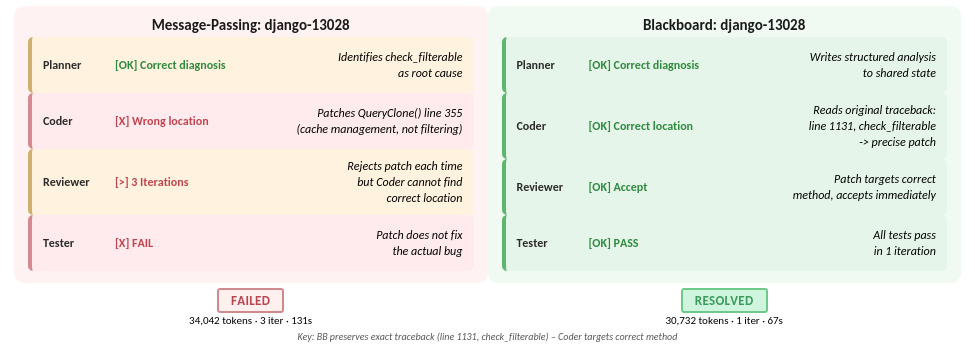
\includegraphics[width=\textwidth]{figures/fig5_information_flow_regenerated.png}
\caption{Case study: django-13028. Under MP, the Planner's compressed summary omits precise location details, causing the Coder to patch the wrong method. Under BB, direct access to the original issue traceback enables a correctly targeted one-iteration fix.}
\label{fig:case-study}
\end{figure*}

\textbf{MP Failure}: The Planner correctly identifies the root cause---a naming collision between a user-defined filterable field and Django's internal \texttt{check\_filterable} method. However, its summary compresses the diagnosis into approximately 679 tokens without exact traceback line numbers or method location (\texttt{Query.check\_filterable} at line 1131 of \texttt{django/db/models/sql/query.py}). Instead, the Coder patches \texttt{Query.clone()} at line 355, which is a different method for managing the query cache. Despite three iterations, the Coder never locates the actual \texttt{check\_filterable} method.

\textbf{BB Success}: The Coder reads the Planner's analysis and the original issue description, which includes the full traceback: File "django/db/models/sql/query.py", line 1131, in \texttt{check\_filterable}. With direct access, the Coder generates a precisely targeted one-iteration patch adding a \texttt{hasattr(expression, '\_meta')} guard, correctly resolving the issue.

\textbf{Concrete Impact}: MP consumed 34,042 tokens across 3 iterations (131s) and failed; BB consumed 30,732 tokens in 1 iteration (67s) and succeeded. This example illustrates how message passing can introduce information loss during summarization: even when the Planner's diagnosis is correct, the compressed representation may omit the precise location details required for accurate patch generation.

\subsection{Statistical Summary}
\label{sec:stat-summary}

Table~\ref{tab:statistics} consolidates the statistical test results across all comparisons.

\begin{table}[!ht]
\centering
\footnotesize
\caption{Statistical test results. * indicates significance at $\alpha=0.05$.}
\label{tab:statistics}
\begin{tabular}{@{}llrl@{}}
\toprule
\textbf{Test} & \textbf{Comparison} & \textbf{Statistic} & \textbf{p-value} \\
\midrule
McNemar & MP vs BB & $b=1, c=3$ & $p=0.625$ \\
McNemar & MP vs Hybrid & $b=1, c=1$ & $p=1.000$ \\
McNemar & BB vs Hybrid & $b=2, c=0$ & $p=0.500$ \\
Cohen's $h$ & BB vs MP & $h=0.116$ & negligible \\
Odds Ratio & BB vs MP & OR=1.40 & CI [0.45, 4.37] \\
Wilcoxon & Tokens: MP vs BB & $W=34$ & $p<0.001$* \\
Wilcoxon & Tokens: MP vs Hy & $W=183$ & $p<0.001$* \\
Wilcoxon & Latency: MP vs BB & $W=63$ & $p<0.001$* \\
Wilcoxon & IFS: MP vs BB & $W=36.5$ & $p=0.058$ \\
\bottomrule
\end{tabular}
\end{table}

\section{Discussion}

\subsection{The Information Preservation Advantage}

Our results indicate that the Blackboard architecture improves information preservation in multi-agent SE pipelines. The 62\% increase in Coder-stage IFS (0.586 vs. 0.362) suggests that shared-state access helps retain key technical entities more effectively. This observation is consistent with previous work on Blackboard architectures for reasoning systems \cite{wang2025lbmas} and data science workflows \cite{salemi2025llm}, extending these findings to software engineering.

The mechanism behind this improvement follows from the context functions defined in Section~\ref{sec:comm-modes}. Under MP, $I \notin C^{\text{MP}}(\text{Coder})$: the Coder's only source of information about the issue is the Planner's natural language summary $\text{out}(\text{Planner})$, which compresses and paraphrases the original content. Under BB, $I \in C^{\text{BB}}(\text{Coder})$: the Coder has access to both the Planner's structured analysis $A$ and the original issue text $I$, allowing it to cross-reference and recover details that might be absent from the Planner's summary. This architectural guarantee of information access is the fundamental advantage of the Blackboard architecture. The marginal significance ($p=0.058$) with 28 non-zero paired differences suggests that a modestly larger experiment ($\sim$35--40 pairs) could yield $p<0.05$.

We argue that \textbf{IFS and file targeting---not resolve rate---constitute the primary empirical contributions} of this study. Resolve rate is a coarse binary outcome that can be influenced by downstream bottlenecks beyond the communication layer's control. IFS and file targeting isolate the pipeline stages that the communication architecture directly affects, providing a more precise and actionable signal. The 27.5 percentage-point file targeting advantage (82.6\% vs. 55.1\%) is a large and practically meaningful effect that would benefit downstream patch generation methods.

\subsection{Why Is the Resolve Rate Difference Limited?}
\label{sec:resolve-rate-limited}

A central question is the gap between the large IFS improvement (62\%) and the modest resolve rate gain (4pp). The patch quality analysis (Section~\ref{sec:patch-quality-analysis}) together with the tool use ablation (Section~\ref{sec:tool-ablation-study}) reveal a consistent causal chain, which we formalize as an \emph{information flow bottleneck model} (Figure~\ref{fig:bottleneck}):

\begin{enumerate}
\item \textbf{Upstream: BB significantly outperforms MP.} BB achieves a 62\% higher IFS, corresponding to a 27.5pp advantage in correct file targeting (82.6\% vs. 55.1\%).

\item \textbf{Downstream: A systematic bottleneck limits all modes.} Once the correct file is identified, all modes achieve $\sim$22\% conditional resolve rate. The LLM's inability to reliably generate context-correct unified diffs is a limiting factor largely independent of the communication architecture.

\item \textbf{Tool use does not resolve the bottleneck.} Despite file access and \texttt{validate\_patch} capability, the LLM cannot generate corrected patches (Section~\ref{sec:tool-ablation-study}). Token consumption increases 2--4x without improving resolve rates.

\item \textbf{The bottleneck attenuates upstream advantages.} BB's 27.5pp file-targeting advantage translates to approximately $27.5 \times 0.22 \approx 6$ additional resolve-rate percentage points in expectation---close to the observed 4pp gain.

\end{enumerate}
These findings suggest that BB's observed advantage closely matches what would be expected under the downstream bottleneck. As LLM diff-generation capabilities improve, or alternative patch representations bypass this constraint, the upstream advantages of BB may translate more fully into improvements in resolve rate.

The predictive accuracy of this model deserves emphasis. From BB's 27.5pp file-targeting advantage and the $\sim$22\% conditional resolve rate, the model predicts an expected improvement in resolve rate of $27.5 \times 0.22 \approx 6$pp. The observed gain is 4pp (16\% vs. 12\%), falling within the expected range given sampling variance on 50 issues. This correspondence between predicted and observed effects provides strong internal validity for the bottleneck model, regardless of whether the difference in resolve rates itself is statistically significant.

\textbf{A note on statistical power.} A post-hoc power analysis indicates that detecting a 4 percentage-point difference (12\% vs. 16\%) using McNemar's test at $\alpha = 0.05$ with 80\% power would require approximately $N = 300$ paired observations, roughly six times the size of our sample. Accordingly, this study was not designed to establish statistical significance for resolve rate alone. Instead, resolve rate is interpreted as one component of a multi-metric evaluation strategy, where IFS ($p = 0.058$), file targeting (+27.5pp), the bottleneck model, the tool-use ablation, and the case study together support a consistent explanation. We view this convergence of evidence as more informative than any single p-value.

\subsection{Why Does Hybrid Not Outperform?}

The Hybrid configuration (12.0\%) matches MP rather than exceeding BB. This pattern can be explained by the context functions defined in Section~\ref{sec:comm-modes}: $C^{\text{Hy}}$ is a strict superset of both $C^{\text{MP}}$ and $C^{\text{BB}}$, combining the predecessor's natural-language output with the full shared state. When presented with this larger context---consistent with prior findings that LLMs struggle to make effective use of very long inputs \cite{liu2024lost}---the Coder often produces no diff output. Specifically, 36\% of Hybrid runs generate empty patches (18/50), compared with 2\% for MP and 8\% for BB.

However, among non-empty patches, Hybrid achieves a file-targeting rate of 78.1\%, close to BB's 82.6\%, and its conditional resolve rate (24.0\%) is the highest among the three configurations. These results suggest that the limitation arises from input format and context size, rather than insufficient information quality. Therefore, future hybrid designs may benefit from mechanisms that limit context overload, such as selective sharing or progressive disclosure.

\subsection{Implications for Practice and System Design}

\textbf{Adopt shared state for long pipelines.} The information-preservation advantage of BB is likely to increase as pipeline length grows, because each MP handoff introduces an additional compression step. For pipelines with two or more stages, a shared-state design may therefore be a sensible default architectural choice.

\textbf{Communication and code generation are orthogonal concerns.} Communication architecture optimization (upstream: information preservation, file targeting) and code generation optimization (downstream: patch correctness) address different stages of the pipeline. Systems should adopt Blackboard for upstream quality while investing separately in downstream improvements---such as alternative patch representations, retrieval-augmented generation \cite{lewis2020retrieval} for context lines, or model fine-tuning for diff generation. The combination is expected to be multiplicative.

\textbf{IFS as a diagnostic metric.} IFS provides stage-by-stage diagnostics that are independent of task success. Despite similar resolve rates, IFS differences reveal information-quality gaps that may become significant as other bottlenecks are addressed.

\textbf{Avoid naive hybrid designs.} Combining communication channels without careful integration may reduce performance, as illustrated by the 36\% empty-patch rate observed in the Hybrid configuration.

\subsection{Beyond Resolve Rate: A Case for Multi-Metric Evaluation}

A reviewer might ask: if resolve rate is not statistically significant, what has this study demonstrated? We argue that evaluation in multi-agent SE systems should not rely solely on end-to-end binary outcomes. Resolve rate collapses the entire pipeline into a single binary indicator, making it insensitive to improvements at individual stages when failures in other stages dominate the overall outcome. In our experiments, 86--88\% of runs fail during patch application regardless of communication mode, creating a noise floor that obscures upstream improvements.

Our multi-metric evaluation decomposes the pipeline into measurable stages. IFS captures information preservation, file targeting measures code localization accuracy, and conditional resolve rate reflects patch generation precision. This decomposition shows that BB substantially outperforms MP on the stages it is intended to affect (IFS: +62\%, file targeting: +27.5pp), while the stage it does not influence---patch generation---remains limited, with a roughly 22\% conditional resolve rate across all configurations. Without this decomposition, one might conclude that communication architecture has little effect, when in fact it improves the stages it directly influences while a downstream bottleneck constrains the final outcome.

These findings suggest that future evaluations of multi-agent SE systems would benefit from similar decomposition strategies that report intermediate metrics alongside end-to-end results. Such reporting enables meaningful comparisons even when sample sizes are insufficient to detect statistically significant differences in final outcomes. It also provides clearer guidance about which stages of the pipeline require improvement.

\section{Threats to Validity}
\label{sec:threats}

\textbf{Internal Validity.} We use a single LLM (Claude Sonnet 4.5) with temperature set to 0. This design choice removes model-related variance as a potential confounding factor, ensuring that observed differences across configurations can be attributed to the communication architecture rather than to variation in model behavior. The trade-off is reduced generalizability: the exact magnitude of the observed improvements (e.g., IFS gains or differences in resolve rates) may vary across models \cite{brown2020language}. However, the underlying direction of BB's advantage---improved information preservation through shared-state access---is an architectural property that does not depend on a specific LLM. The sequential pipeline also introduces an ordering effect, where a weak Planner analysis can influence all downstream agents regardless of communication mode. To reduce this effect, we use identical Planner prompts across all configurations.

\textbf{External Validity.} Our sample of 50 issues from SWE-bench Lite is limited to well-maintained Python repositories. Django issues are overrepresented (22/50), and because BB's resolve-rate advantage is concentrated in easy Django issues, the observed effect may partly reflect repository-specific factors, such as Django's detailed issue descriptions and well-structured codebase. As a result, the findings may not generalize to other programming languages, less-documented repositories, or software engineering tasks beyond bug fixing. However, the IFS advantage appears consistently across all repositories in our sample, not only Django, suggesting that the underlying information-preservation mechanism is not tied to a particular repository.

\textbf{Construct Validity.} IFS relies on rule-based entity extraction, which may fail to capture semantically equivalent references or may count incidental mentions as evidence of preservation. As discussed in Section~\ref{sec:resolve-rate-limited}, resolve rate alone may underestimate the effect of communication architecture. The intermediate metrics used in this study provide a more complete assessment.

\textbf{Statistical Validity.} With 50 issues and only 4 discordant pairs, McNemar's test has limited statistical power to detect the observed 4 percentage-point difference in resolve rate. A post-hoc power analysis indicates that $N \approx 300$ paired observations would be required to detect a difference of this magnitude with 80\% power at $\alpha = 0.05$. The IFS result ($p = 0.058$) is close to, but does not reach, the conventional significance threshold. To mitigate the risk of overinterpreting p-values under limited sample size, we report effect sizes and confidence intervals alongside hypothesis tests. These statistics provide a more stable characterization of the observed differences and facilitate comparison with future studies.

\section{Conclusion and Future Work}

\subsection{Conclusion}

This paper introduced SE-Blackboard, applying the Blackboard shared-state architecture to multi-agent software engineering pipelines. Through controlled experiments on 50 SWE-bench Lite issues, we show that communication architecture measurably affects information preservation and intermediate task performance. Our main findings are:

\begin{enumerate}
\item \textbf{Information Preservation}: BB improves Coder-stage IFS by 62\% compared with MP (0.586 vs. 0.362, $p = 0.058$), indicating that shared-state access substantially reduces information loss across pipeline stages.

\item \textbf{Code Localization}: BB's information advantage translates into 82.6\% correct file targeting versus 55.1\% for MP, improving the key prerequisite for successful patch generation.

\item \textbf{Information Flow Bottleneck Model}: Once the correct file is identified, all configurations converge to a $\sim$22\% conditional resolve rate, indicating that LLM diff-generation reliability currently limits end-to-end performance. A tool-use ablation further shows that this bottleneck cannot be removed through tool access alone.

\item \textbf{Resolve Rate}: BB achieves a 16.0\% resolve rate compared with 12.0\% for MP (a 33\% relative improvement), consistent with the bottleneck model's prediction that a 27.5pp file-targeting advantage should yield roughly 6pp expected improvement in resolve rate.

\item \textbf{Hybrid Caution}: Directly combining communication channels can degrade performance due to context overload, producing a 36\% empty-patch rate, although successful Hybrid patches achieve file-targeting accuracy close to BB.

\end{enumerate}
These results highlight communication architecture as an important design dimension for multi-agent SE systems. The proposed information flow bottleneck model further provides a conceptual framework for understanding how improvements in upstream information quality translate into downstream task outcomes.

\subsection{Future Work}

\textbf{Alternative Patch Representations.} The unified diff bottleneck is not resolved through tool augmentation alone. Future work could explore patch representations that avoid strict context-line matching, such as search-and-replace specifications, AST-level edits, or whole-file rewriting.

\textbf{Improved Diff Generation.} Improving diff generation itself is another promising direction. Potential approaches include fine-tuning on patch corpora, constrained decoding for diff syntax, or retrieval-augmented generation \cite{lewis2020retrieval} to retrieve accurate context lines while retaining the unified diff format.

\textbf{Debate Topology.} The SE-Blackboard framework also supports a debate-style topology in which multiple Coders generate competing patches and a Reviewer selects the best candidate. Prior work shows that multi-agent debate can improve factuality and reasoning in LLMs \cite{du2024improving}. Evaluating this topology across different communication architectures would help determine whether the benefits of shared state compound as agent diversity increases.

\textbf{Larger-Scale Evaluation.} Future studies should extend the evaluation to the full SWE-bench Lite dataset (300 issues) and include multiple LLMs. Such experiments would provide sufficient statistical power for resolve rate comparisons and allow stronger conclusions about generalizability.

\textbf{Broader Applications.} The Blackboard architecture may benefit other software engineering tasks, such as feature development, code review, and test generation, as well as domains that require precise information transfer in multi-agent systems.

\section*{Data and Code Availability}

The source code for the SE-Blackboard framework is publicly available on GitHub at \url{https://github.com/el4435/SE-Blackboard} and archived as an executable capsule on Code Ocean. The experiment data, including all result files, statistical analyses, and figures, are available on Zenodo at \url{https://doi.org/10.5281/zenodo.18911615}.

\section*{Acknowledgment}

Large language models were used during the preparation of this work. ChatGPT was used to assist with proofreading and language editing of the manuscript, and Claude was used to assist with portions of the implementation. The authors reviewed all outputs and take full responsibility for the design, analysis, and conclusions presented in this paper.

\bibliographystyle{IEEEtran}
\bibliography{references}

\begin{IEEEbiography}[{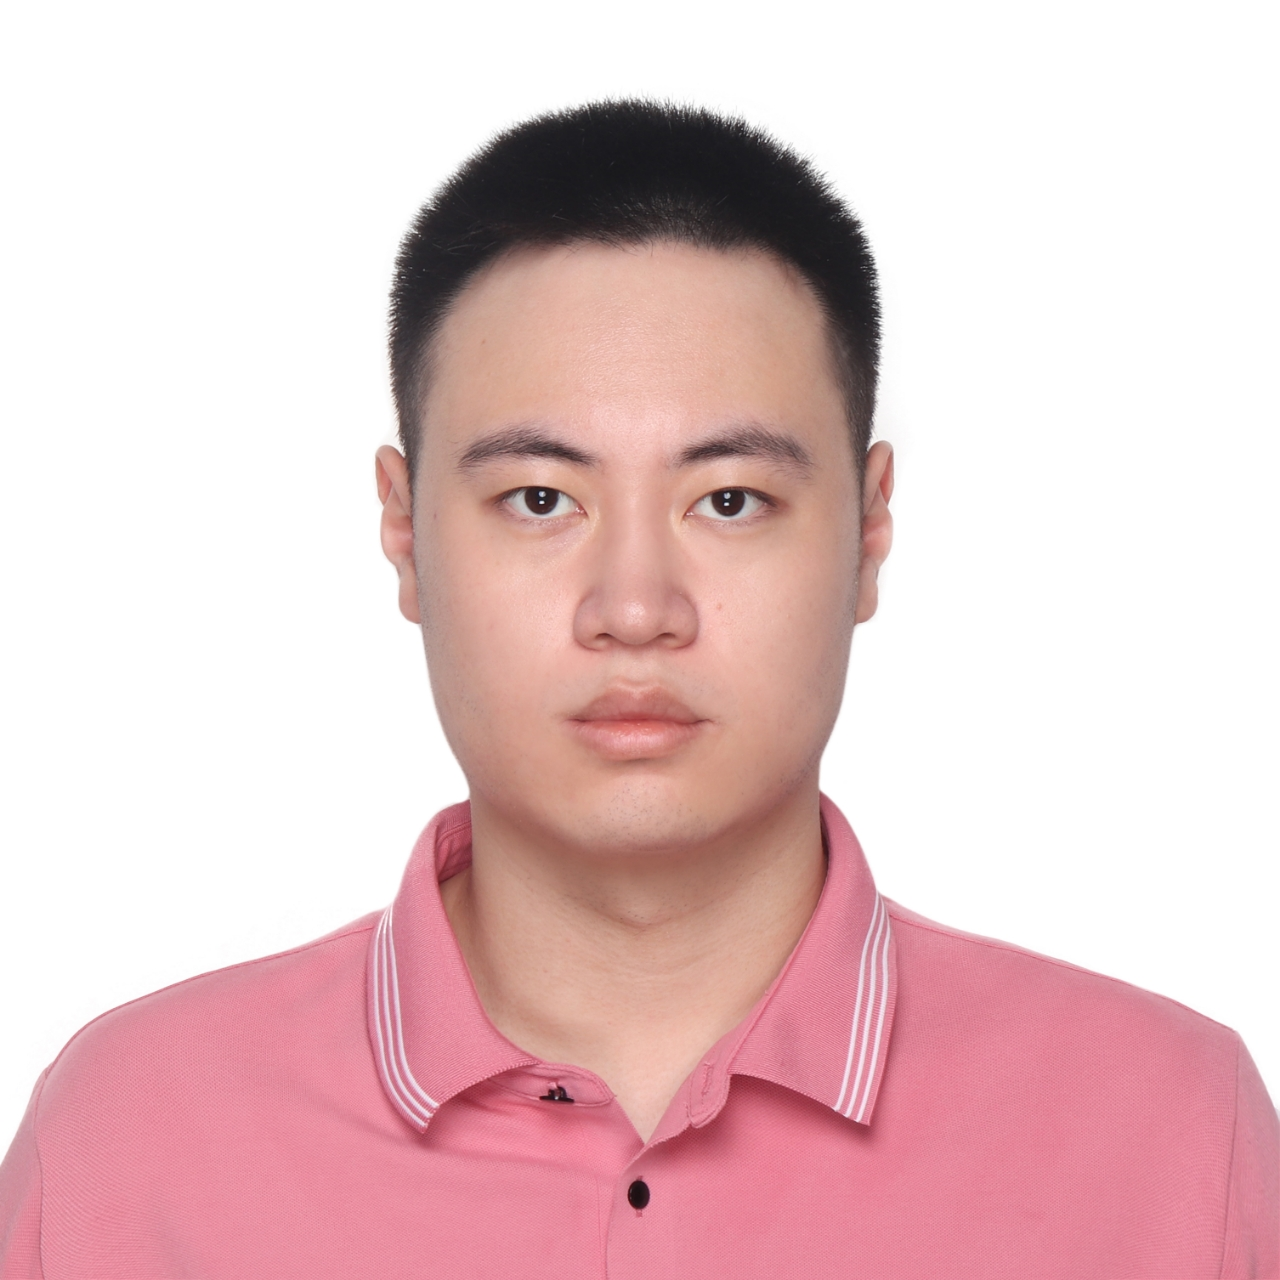
\includegraphics[width=1in,height=1.25in,clip,keepaspectratio]{author_liu.jpg}}]{Erxi Liu} received the B.S. degree in computer science from Syracuse University, Syracuse, NY, USA, in 2022. He is currently pursuing the M.S. degree in computer engineering at the Tandon School of Engineering, New York University, New York, NY, USA. He was previously with ZTE Corporation, where he worked on intelligent operations and maintenance (AIOps). He was also a Research Intern with the Chinese Academy of Sciences, focusing on operating system migration for robotic frameworks, and with Zhejiang Dajingyi Lean Co., Ltd., where he developed AI-based algorithms for industrial pipeline inspection. His experience spans both industry and research across software systems and applied AI. His research interests include multi-agent systems, large language models, software engineering automation, AI-driven DevOps, and human--AI collaboration.
\end{IEEEbiography}

\begin{IEEEbiography}[{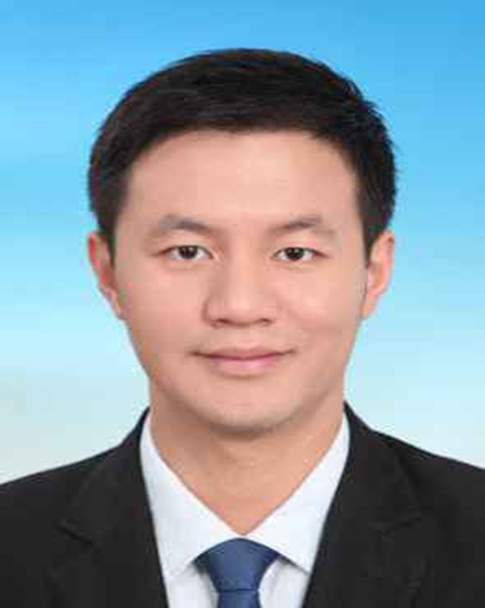
\includegraphics[width=1in,height=1.25in,clip,keepaspectratio]{author_zhu.png}}]{Qiang Zhu} received the Ph.D. degree in optical engineering from the University of Chinese Academy of Sciences, Beijing, China, in 2022. He is currently an Associate Researcher and Master's Supervisor at the National Institute of Metrology, China, where he serves as the Head of the Optical Rotation Metrology Laboratory. He is a registered expert and member of ISO/TC 130 and a member of the National Printing Machinery Standardization Technical Committee. He also serves as a Master's Supervisor at Beijing Institute of Graphic Communication and Xi'an University of Technology. He has participated in six national key projects, including the National Key R\&D Program, and has led the drafting of two national standards. He has received one first prize and two third prizes at the provincial and ministerial level for scientific and technological achievements. He has published over 20 academic papers, with more than three indexed by EI. His research interests include photoelectric precision instruments, photoelectric detection technologies, and optical rotation metrology.
\end{IEEEbiography}

\begin{IEEEbiography}[{
\includegraphics[width=1in,height=1.25in,clip,keepaspectratio]{author_dong.jpg}}]{Xinru Dong} received the B.S. degree from Mudanjiang Normal University, Mudanjiang, China, in 2023. She is currently pursuing the M.S. degree at the School of Mechanical and Electrical Engineering, Beijing Institute of Graphic Communication, Beijing, China. She is also a Visiting Student with the Division of Dimensional Metrology, National Institute of Metrology, China, where she participates in research on precision measurement and intelligent instrumentation. Her research interests include dimensional metrology, AI-assisted measurement systems, multi-agent systems, and the application of large language models to engineering workflows.
\end{IEEEbiography}

\EOD

\end{document}
